\documentclass[english,10pt]{article}
\usepackage[a4paper, margin={3cm}]{geometry}
\usepackage[utf8]{inputenc}
\usepackage[T1]{fontenc}
\usepackage{makecell}
\usepackage{lastpage}
\usepackage{fancyhdr}
\usepackage{graphicx}
\usepackage{tabularx}

\usepackage{hyperref}
\pagestyle{fancy}
\title{Curriculum Vitae}
\author{Tobias Hochreiter}
\begin{document}
	\cfoot{\thepage\ / \pageref*{LastPage}}
	\vspace*{-1.5cm}
	%\hrule
	\begin{picture}(0,0)
		\put(330,-110){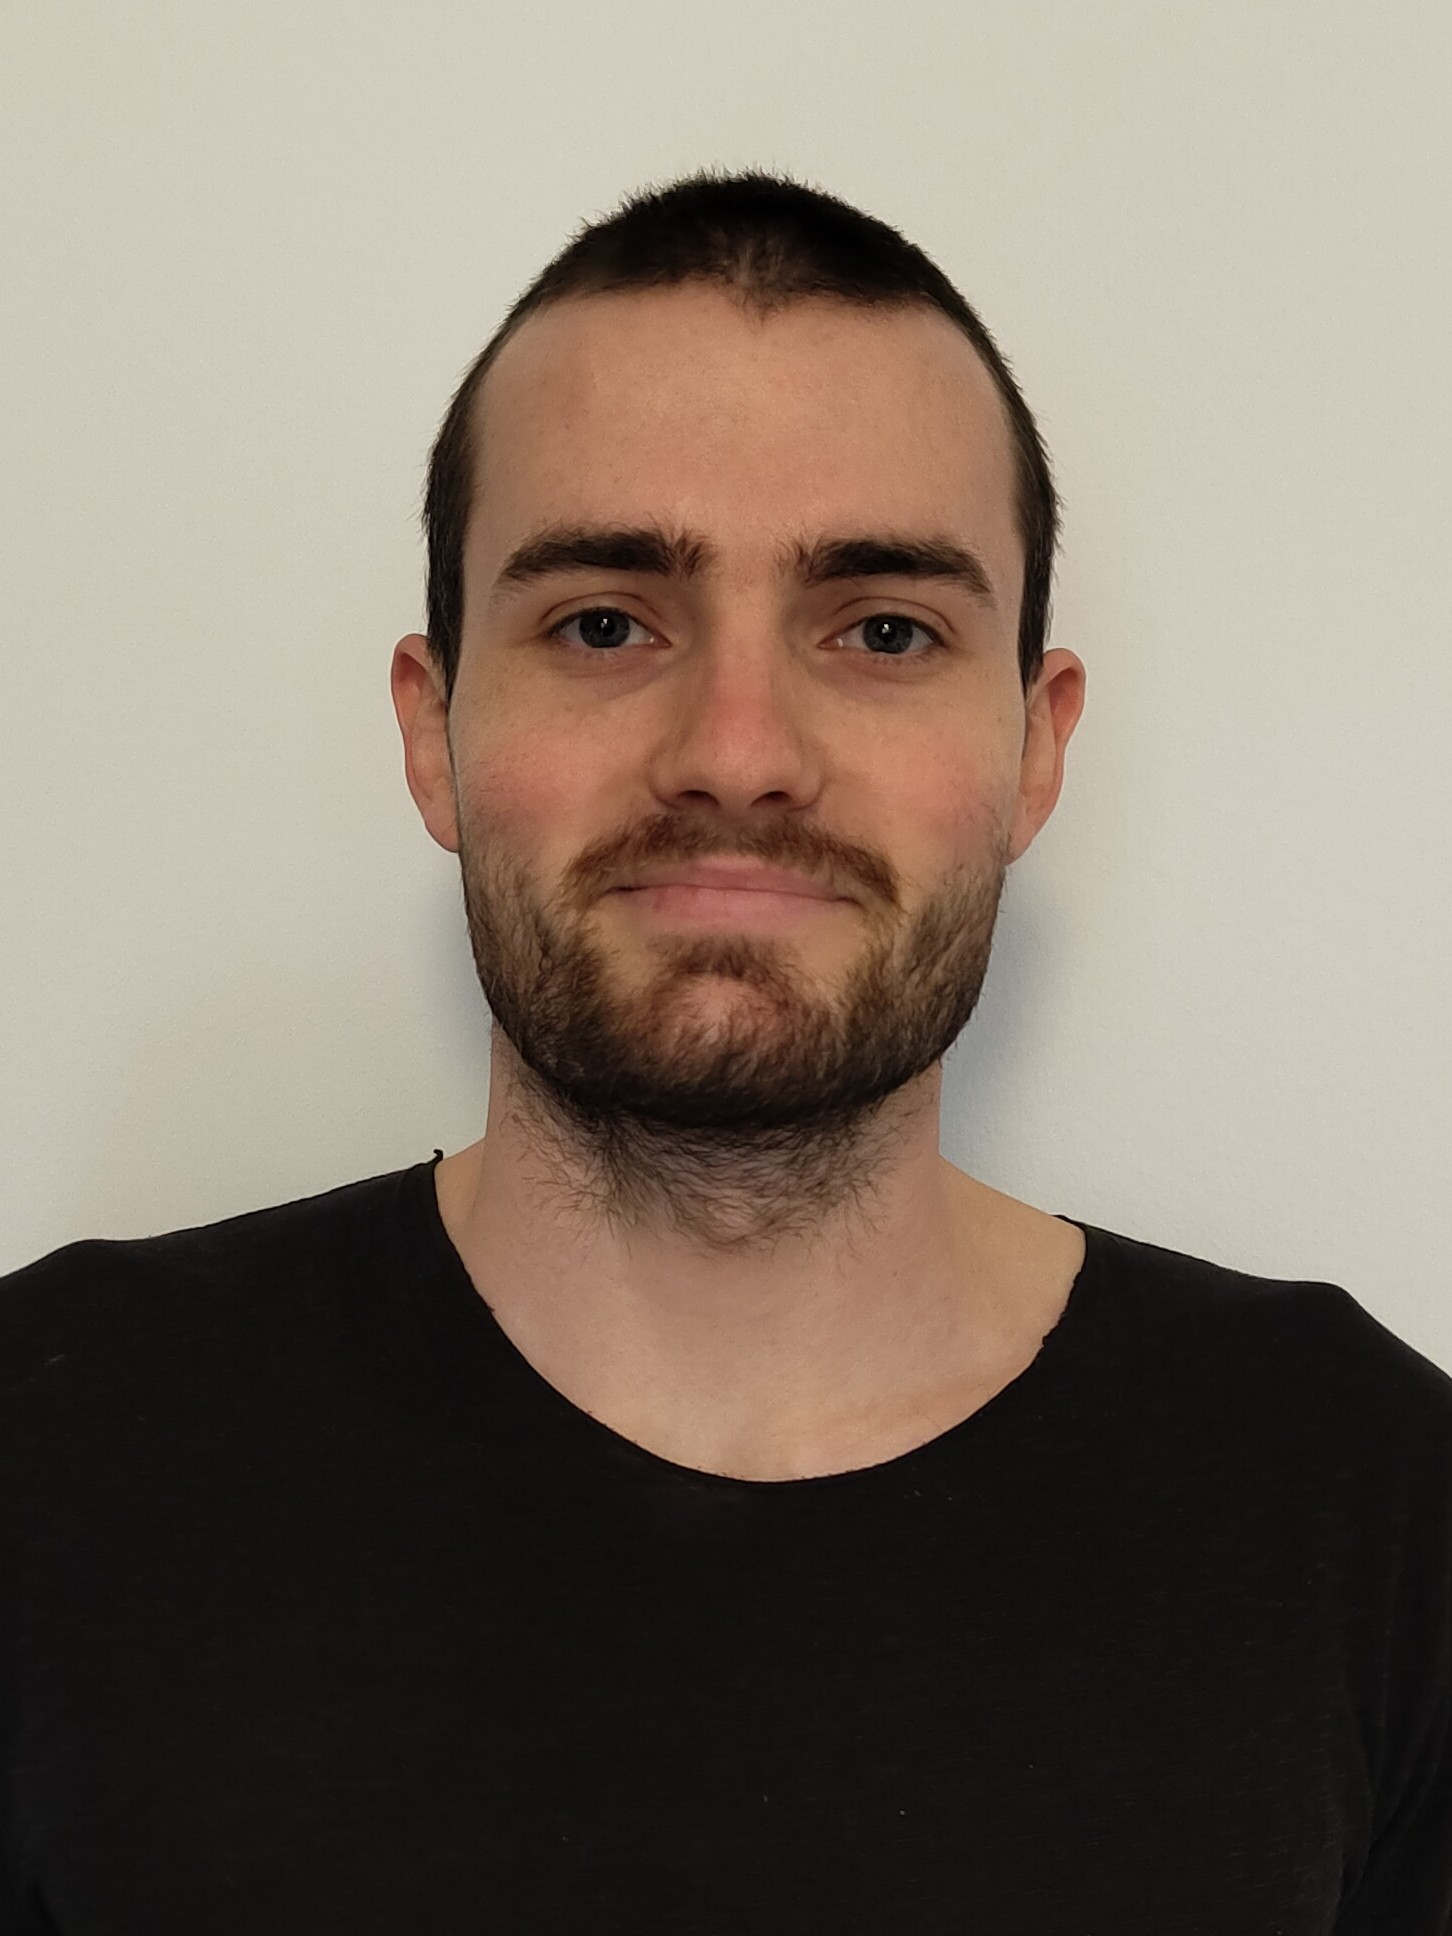
\includegraphics[width=2.8cm]{../moi2.jpg}}
	\end{picture}
	\begin{center}
		\textbf{\LARGE Curriculum Vitae}\\
		\vspace{.4cm}
		{\large Tobias Hochreiter}\\
		\vspace{.2cm}
		tobias.hochreiter@gmx.at
		\vspace{-.5cm}
	\end{center}
	\section*{Personal Data}
	born 10/10/1997 in Salzburg, Austrian citizen, father of 1
		
	\section*{Education \hfill\small(theses at \href{https://github.com/tob-asco/theses}{github.com/tob-asco/theses})}
	\begin{tabularx}{\linewidth}{m{3cm}|X}
		04/2021 - 06/2023 & \makecell{\textbf{\href{https://www.math.uni-hamburg.de/master/mphys/}{UHH}} (Hamburg): M.Sc. Mathematical Physics\\
            \textit{On Topological Quantum Field Theories}}\hfill($1.0$~s.c.l.)\vspace{3pt}\\\vspace{1pt}
		10/2017 - 06/2021 & \makecell{\textbf{\href{https://www.ph.tum.de/academics/bsc/}{TUM}} (Munich): B.Sc. Physics\\
			\textit{Physical and Geometrical Viewpoints of the KdV Equation}}\hfill($1.3$~c.l.)\vspace{3pt}\\\vspace{1pt}
		09/2011 - 05/2016 & \href{http://www.htl-salzburg.ac.at/biomedizin-gesundheitstechnik.html}{HTL Bio-engineering} (Salzburg): A-levels\hfill ($1.4$~s.c.l.)\vspace{3pt}\\\vspace{1pt}
		09/2007 - 07/2011 & \href{https://www.werkschulheim.at}{Werkschulheim Felbertal}
	\end{tabularx}
	
	\section*{Employments}
	\begin{tabularx}{\linewidth}{m{3cm}|X}
        12/2023 - 03/2025 & kids' bouldering guide at \href{https://www.boulderwelt-muenchen-ost.de/}{Boulderwelt München Ost} \hfill(10h/w)\\
		10/2022 - 04/2023 & tutor for \textit{analysis 3 for physicists} \hfill(4h/w)\\
		10/2020 - 04/2021 & tutor for \textit{theo. physics: statistical mechanics}\hfill (8h/w)\\
		04/2020 - 10/2020 & tutor for \textit{theo. physics: quantum mechanics} \hfill (8h/w)\\
		10/2019 - 04/2020 & tutor for \textit{theo. physics: electrodynamics} \hfill (8h/w)\\
		04/2019 - 10/2019 & tutor for \textit{theo. physics: classical mechanics} \hfill (8h/w)\\
		12/2014 - 04/2017 & electric draughtsman at \href{https://www.ib-krallinger.com/}{IB-Krallinger} \hfill ($\sim$6h/w)\\
		10/2013 - 07/2014 & building switchboxes at AML Elektrotechnik \hfill ($\sim$4h/w)
	\end{tabularx}
	
	\section*{Misc. Occupations}
	\begin{tabularx}{\linewidth}{m{3cm}|X}
		since 11/2023 & parental leave\\
		05/2017 - 08/2017 & electronic engineer for circuitry at \href{https://www.die-salzburger-industrie.at/unternehmen/a-b-mikroelektronik-gmbh/}{AB Mikroelektronik} \hfill (internship)\\
		08/2016 - 04/2017 & paramedic \& driver at \href{https://www.roteskreuz.at/salzburg/ich-will-helfen/zivildienst}{Red Cross Salzburg} \hfill  (Civilian Service)\\
		08/2014 - 09/2014 & electric engineer on site at \href{https://www.northdata.com/AML+Elektrotechnik+GmbH,+Koppl/360865i}{AML Elektrotechnik} \hfill (internship)\\
		07/2013 - 08/2013 & hospital in dpt. \textit{medical technology} at \href{https://salk.at/}{SALK} \hfill (internship)\\
	\end{tabularx}
	
	\section*{Scholarships}
	\begin{tabularx}{\linewidth}{m{3cm}|X}
		10/2018 - 10/2023 & \href{https://www.elitenetzwerk.bayern.de/start/foerderangebote/max-weber-programm}{Max Weber-Programm} \hfill (non-material \& 215€/month)\\
		05/2021 - 05/2022 & \href{https://www.qu.uni-hamburg.de/}{Quantum Universe Cluster of Excellence} \hfill (861€/month)
	\end{tabularx}
	
	\section*{Languages}
	\begin{tabular}{m{3cm} | l}
		German & mother language\\
	English & level C1 approx., from higher studies\\
	French & level B2 from \textit{DELF}-exam\\
	Mathematics & mainly algebraic (e.g. category theory) but also analytic (e.g. PDEs)\\
	\textbf{C\#} & cf. \href{https://github.com/tob-asco/seeds}{\texttt{github.com/tob-asco/seeds}}\\
        \LaTeX & author of package \href{https://github.com/tob-asco/counttherefs.git}{\texttt{counttherefs}} and \href{https://github.com/tob-asco/cascade.git}{\texttt{cascade}}\\
	misc. & Linux, Python, XAML, HTML, VB, C++
	\end{tabular}
    \vfill
	\hrule
\end{document}
